% BEGIN TEMPLATE
\documentclass{article}
\usepackage{graphicx}
\usepackage{hyperref} 
\usepackage{xcolor}
\usepackage{nameref}
\usepackage{listings}
\usepackage{float}
\usepackage[title]{appendix}
\usepackage[ruled]{algorithm2e}
\usepackage{fixltx2e}
\graphicspath{ {../../images/} }
\bibliographystyle{acm}
% CHANGE THESE
\newcommand{\courseListing}{CSCI 8150}
\newcommand{\courseName}{Advanced Computer Architecture}
\newcommand{\assignmentTitle}{Final Exam}
\newcommand{\assignmentSubtitle}{Paper Summary and Problem Solutions}
\usepackage{geometry}
\geometry{margin=1in}
\renewcommand{\baselinestretch}{1.2}


\hypersetup{
    colorlinks,
    linkcolor={red!50!black},
    citecolor={blue!50!black},
    urlcolor={blue!80!black}
}
\urlstyle{same}
\definecolor{codegreen}{rgb}{0,0.6,0}
\definecolor{codegray}{rgb}{0.5,0.5,0.5}
\definecolor{codepurple}{rgb}{0.58,0,0.82}
\lstdefinestyle{mystyle}{
    commentstyle=\color{codegreen},
    keywordstyle=\color{magenta},
    numberstyle=\tiny\color{codegray},
    stringstyle=\color{codepurple},
    basicstyle=\ttfamily\footnotesize,
    breakatwhitespace=false,         
    breaklines=true,                 
    captionpos=b,                    
    keepspaces=true,                 
    numbers=left,                    
    numbersep=5pt,                  
    showspaces=false,                
    showstringspaces=false,
    showtabs=false,                  
    tabsize=2
}

\lstset{style=mystyle}

\begin{document}
  \begin{center}
  
\includegraphics[scale=0.15]{UNO-Logo-Color.png}
  \\[0.3in]
  \textbf{\courseListing{}}\\
  \courseName{}
  \\[0.75in]
  \textbf{\assignmentTitle{}}\\
  \assignmentSubtitle{}
  \\[0.75in]
  \textbf{Patrick Davlin}
  \\[0.75in]
  \textbf{Computer Science Department}\\
  \textbf{Peter Kiewit Institute}\\
  \textbf{University of Nebraska}
  \\[0.75in]
  \textbf{Spring 2021}
  \\[0.3in]
  
\includegraphics[scale=0.075]{UNO-Icon-Color.png}
  \newpage
\end{center}
  \graphicspath{{./images/}}
% END TEMPLATE

\section{Summary of \textit{Shared Memory Consistency Models: A Tutorial}}
\subsection{Introduction and Uniprocessor Baseline}

\par At the highest level, the paper \textit{Shared Memory Consistency Models: A Tutorial} covers the problem of memory consistency in multiprocessor systems.
Put simply, the general problem is similar to problems covered in class, where one processor might access a specific field of shared data, observing old or incorrect (strictly in terms of the programmatic flow) data prior to completion of some unrelated operation from a different processor.
This is a critical issue to address from a systems perspective, because programmers may not be able to solve the problem on their own without introducing timing uncertainty to processes.
Moreover, allowing programs to assume that the memory they get is correct aids in making programs universal, which is to say that a program \textit{should} be able to run the same way on any system, regardless of the specific architecture of its processors and memory.

\par To establish a comparison point for the consistency models in multiprocessor systems, the authors first discuss memory semantics in uniprocessor systems.
This is intuitive--when memory operations occur in a uniprocessor system, they occur in program order, so that any instructions executed in the same location happen sequentially.
It also allows for many of the conventions associated with processor systems--pipelining, loops, and lockup-free caches, to name some.

\subsection{Sequential Consistency}

\par Having established a baseline behavior and programmer expectation for how memory operations behave, the authors go on to outline models for replicating these expectations in multiprocessor systems.
The first such model is \textit{sequential consistency}, which is fundamentally a method to ensure that program order is maintained by a memory system for individual processors while also establishing a single order for all instructions being processed, across all processors.
This provides the appearance of atomic execution, allowing different processes to execute reliably and have their changes reflected across the entire system, simultaneously. The authors go on to describe implementation optimizations, and their associated problems for sequential consistency, in a few common hardware configurations. 

\par The first configuration covered is \textbf{Architectures Without Caches}.
The authors outline a handful of ways that a multiprocessor architecture can violate memory consistency without use of a cache.
In general, these are all related to the timing of read or write propagation.
If a processor needs to read data from some memory location, and that memory location has an outdated or incorrect memory value as a result of a different processor's delayed write process, the computer no longer respects program order.
There are three causes of this exact behavior--write buffers, overlapping write operations, and non-blocking read operations--but they all contribute to the core issue of \textit{read operations occurring before write operations}, which leads to a violation of sequential consistency.

\par Having established possible sequential consistency violations in hardware optimizations for architectures without caches, the authors move on to discuss \textbf{Architectures with Caches}.
Caching provides general protections for frequently-accessed memory locations, but its associated optimizations each present the possibility of sequential consistency violations.
In general, the protections offered by caches alleviate the timing problems encountered by architectures that lack them, but alone, are not enough to guarantee that writes to the same location would be serialized in implementation.
To start, the principle of cache coherence requires that all writes to the same location be made visible to all processors, and that those write operations are \textit{seen} in the same order by all processors, but does not guarantee that writes to \textit{all} locations are seen in the same order by \textit{all} processors.
This distinction is important because a cache system is focused on maintaining the integrity of memory locations, but sequential consistency is concerned with ensuring the integrity of a program acting upon those systems.

\par Multiprocessor systems with caches also provide acknowledgement to processors that write operations are completed.
Like cache coherence, this alone is not enough to guarantee that write order is protected unless the cache is also propagating those acknowledgements to all processors.
If not, the problem is functionally the same as overlapping write operations in a cache-less system; acknowledging a write completion to one processor does not guarantee that another processor's cache copy has been updated with that data as well.
As a solution to maintain sequential consistency, the authors propose that caches extend this acknowledgement to a second tier; whenever a processor executes a write operation, the system should gather acknowledgements from all cache modules that the write has been completed, and only then notify the writing processor that the write operation has been completed.

\par Sequential consistency requires that write operations appear atomic (that they execute in order) to the processor, but the underlying mechanics of that are often not atomic.
To prevent reads in different processor from receiving values out of order, writes to the same location should be ordered such that processes reading from that value receive the correct value in program order.
To prevent processors from seeing the same write operation to a location at different times, cache copies should acknowledge their receipt of the invalidate or update message from that write operation before more instructions are executed.

\par Finally, the authors note that characteristics of a system may not be isolated solely to hardware, but may exist in the compiler of a uniprocessor system as well.
The principles outlined above, in terms of sequential consistency, apply not strictly to \textit{processors} but to the \textit{processes} being executed simultaneously in any system.

\par An interesting trait of the sequential consistency principle is the extent to which it constrains many of the optimizations that can be applied to multiprocessor systems.
It is fairly obvious to say that this concept is central to the implementation of multiprocessor systems.
The fact that many computer scientists and industry software engineers have not ever needed to consider the core concept of sequential consistency in order to write effective code speaks to the criticality of properly implementing this concept in modern systems.
The paper does an excellent job of clarifying this in terms that are understandable.

\subsection{Relaxed Memory Models}\label{relaxed}
\par The paper provides the characteristics of systems with more relaxed memory models, in contrast to the principles outlined above.
Generally speaking, there are three "buckets" of relaxations for these models: relaxation of program order, ability for a processor to read others' write operations early, and ability for a processor to read its own write operation early.
These relaxations variously impact program order and write atomicity, and in most cases, can be overridden in the scope of a model for greater protections as needed by a program.
The authors list eight system models that all apply various relaxations from sequential consistency.
For each relaxation, the authors describe various methods that models uses to implement them, where applicable.

\par Relaxation of program order can broadly be further broken down further into three categories. 
The first of these involves relaxing the program order for read operations that immediately follow write operations, provided the read operation is for a different location.
In general, this is safe, but exposes the system to risk that sequential consistency be violated along the lines of a write buffer error.
Depending on the implementation, each model may strictly isolate this behavior to single processors, not allowing any read to proceed until the value of a write is visible to all processors (IBM 370 model); allowing a processor to read the value of its own write before it is visible to other processors (TSO); or allow a read value to return the value of any write operation before it is made visible to all processors (PC model).
Safety nets can be implemented by the programmer for TSO and PC by replacing read or write instructions with read-modify-write instructions, which would allow for program order to be maintained.
Similarly, for atomicity, TSO requires a read-modify-write safety net, while PC and 370 do not.
This relaxation can dramatically improve performance if implemented on a hardware level, but is unlikely to have the same impact to a compiler.

\par The second program order relaxation is for write to read and write to write orders.
Only one model (PSO) is listed in the paper with support for this, optimizing write to read operations in a similar manner as TSO but also allowing consecutive write operations to reach memory out of order, ostensibly skipping the time needed to wait on a write cycle to finish before immediately writing again to a different location. As a safety net, the PSO model includes a specific instruction for enforcing program order between writes for situations where the program order needs to be maintained.

\par The third program order relaxation covers all program orders, and has subsets of its own. Weak ordering is the first; it establishes the categories of data operations (reads and writes) and synchronization operations (safety net operations meant to preserve program order). 
The former are associated with a program counter, which increments as they accumulate and decrement as they are completed in order. 
The latter may not be issued until any prior data operations are completed and the counter is zero.

\par The next subset of all-program-order relaxation methods is release consistency. Similar to weak ordering, models that implement release consistency establish two groups of operation types, ordinary and special operations, corresponding roughly to the data and synchronization groups mentioned previously. 
Special operations can also be broken down into "sync" and "nsync" (asynchronous) operations.
Sync operations can \textit{further} be broken down into "acquire" and "release" operations, indicating the availability of resources for synchronous operations.
The two models implementing this approach differ in whether they seek to preserve sequential consistency (RCsc) or processor consistency (RCpc) in the order of special operations.
RCpc requires an implementation of the read-write-modify instruction in a write followed by a read in order to enforce program order and maintain atomicity.
RCsc, on the other hand, preserves atomicity by properly labeling special instructions.

\par The final all-program-order relaxation method, used in the Alpha, RMO, and PowerPC models, uses specific fence instructions as safety nets.
In general, fence instructions cause the processor to enforce sequential consistency on operations before and after the fence instruction.
The Alpha model has two fence instructions to preserve program order for general memory operations and writing instructions, and needs no atomicity safety net.
The RMO model has a fence instruction encoded with four bits to denote which specific program order is being enforced. It, too, does not require a safety net for atomicity.
The PowerPC model has one fence instruction, and that fence instruction can cause consecutive reads to appear out of program order if the fence instruction is placed between them. To maintain atomicity, read-modify-write operations may be needed, since the PowerPC platform allows write operations to be seen by other processor read operations.

\subsection{Abstractions for Relaxed Models}
\par The final main section of the paper addresses the added programmatic complexity of the models described in \nameref{relaxed}.
When programming for different models, it is difficult to account for the differences in behavior when writing a program that needs to execute on multiple machines, and further, difficult to implement the proper safety nets for those systems.
To alleviate this, the authors propose a model by which programmers provide information about their programs to the system, which then determines whether its own optimizations can be applied without compromising the program order of the supplied program.
They call this a "programmer-centric approach," which allows programmers to define their expectations for a program's execution and have those expectations met by the system.

\par The idea of "programmer-centric approach," as an extension the notion of sequential consistency, is mostly taken for granted in 2021 by the common programmer or software engineer.
\textit{Of course} most programmers writing code in a modern system do not actively consider whether that system will execute their instructions in order.
Having the problem solved at a system level as a function of engineering has opened the door for significant strides in programming development over the period of time since this paper's publication, and that progress probably would have been impossible if not for the abstraction of low-level concerns far into the system level.

\newpage

\section{Question 2}
\textbf{Assume that the initial value of r\textsubscript{1}, r\textsubscript{2}, M[a] and M[flag] are 0 upon entry. \textit{BEQZ(r1, L) means jump to label L if r1 is 0. Store(a, 1) means store value 1 in a.}}

    {\centering
        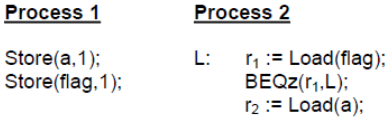
\includegraphics[width=2.5in]{csci-8150/final-exam-1/images/arch_final_2.png}\par 
    }
    
\textbf{A) Assuming sequential consistency (SC) enumerate all possible value pairs of (r\textsubscript{1}, r\textsubscript{2}) after executing the above code.}

\textbf{B) What if we allow re-ordering of loads but not stores? Enumerate all possible value pairs after executing code.}

\newpage
\section{Question 3}

\textbf{Modern microprocessors have store buffers to reduce the latency of store instructions which are often not on the critical path. In these processors, a load instruction first looks up the store buffer to find a match. If there is a match, the value is forwarded from the store buffer; otherwise, the load instruction goes to the data cache. We call this mechanism load-store-optimization. Assume (1) no reordering of load and store instructions within a processor and (2) zero initial values for M[flag1] and M[flag2].}

    {\centering
        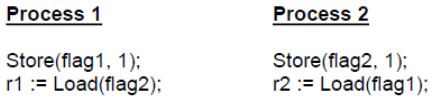
\includegraphics[width=3in]{csci-8150/final-exam-1/images/arch_final_3.png}\par 
    }

\textbf{Suppose your colleague considers a processor with load-store optimization and claims that all four combinations of values of (r\textsubscript{1}, r\textsubscript{2}) pair—i.e., (0, 0), (0, 1), (1, 0) and (1, 1)—are possible after execution of the above code.}

\textbf{A) Explain briefly how each combination can occur (e.g., order of instruction execution, operation of store buffer, etc.). If certain combination cannot occur, justify.}

\textbf{B) Some of IBM 370 families implement load-store optimization. In their implementation, if we insert load instructions (shaded in gray) to part A), one combination gets eliminated from the possible final states of (r\textsubscript{1}, r\textsubscript{2}). (Again, assume (1) no reordering of load and store instructions within a processor and (2) zero initial values for M[flag1] and M[flag2].)}

    {\centering
        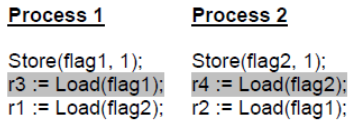
\includegraphics[width=3in]{csci-8150/final-exam-1/images/arch_final_3_2.png}\par 
    }

\textbf{Which combination can be eliminated? From this information, what can you infer about the implementation (or behavior) of the store buffer and short circuits in IBM 370? Explain briefly.}

\end{document}